%%%%%%%%%%%%%%%%%%%%%%%%%%%%%%%%%%%%%%%%%
% University Assignment Title Page 
% LaTeX Template
% Version 1.0 (27/12/12)
%
% This template has been downloaded from:
% http://www.LaTeXTemplates.com
%
% Original author:
% WikiBooks (http://en.wikibooks.org/wiki/LaTeX/Title_Creation)
%
% License:
% CC BY-NC-SA 3.0 (http://creativecommons.org/licenses/by-nc-sa/3.0/)
% 
% Instructions for using this template:
% This title page is capable of being compiled as is. This is not useful for 
% including it in another document. To do this, you have two options: 
%
% 1) Copy/paste everything between \begin{document} and \end{document} 
% starting at \begin{titlepage} and paste this into another LaTeX file where you 
% want your title page.
% OR
% 2) Remove everything outside the \begin{titlepage} and \end{titlepage} and 
% move this file to the same directory as the LaTeX file you wish to add it to. 
% Then add \input{./title_page_1.tex} to your LaTeX file where you want your
% title page.
%
%%%%%%%%%%%%%%%%%%%%%%%%%%%%%%%%%%%%%%%%%
%\title{Title page with logo}
%----------------------------------------------------------------------------------------
%	PACKAGES AND OTHER DOCUMENT CONFIGURATIONS
%----------------------------------------------------------------------------------------

\documentclass[12pt]{article}
\usepackage[english]{babel}
\usepackage[utf8x]{inputenc}
\usepackage{amsmath}
\usepackage{graphicx}
\usepackage{float}
\usepackage[colorinlistoftodos]{todonotes}
\usepackage{hyperref}

\begin{document}

\begin{titlepage}

\newcommand{\HRule}{\rule{\linewidth}{0.5mm}} % Defines a new command for the horizontal lines, change thickness here

\center % Center everything on the page
 
%----------------------------------------------------------------------------------------
%	HEADING SECTIONS
%----------------------------------------------------------------------------------------

\textsc{\LARGE Université Libre de Bruxelles}\\[1.5cm] % Name of your university/college
\textsc{\Large Real-Time Operating Systems }\\[0.5cm] % Major heading such as course name

%----------------------------------------------------------------------------------------
%	TITLE SECTION
%----------------------------------------------------------------------------------------

\HRule \\[0.4cm]
{ \huge \bfseries Mastermind solver}\\[0.4cm] % Title of your document
\HRule \\[1.5cm]
 
%----------------------------------------------------------------------------------------
%	AUTHOR SECTION
%----------------------------------------------------------------------------------------

\begin{minipage}{0.4\textwidth}
\begin{flushleft} \large
\emph{Authors:}\\
ABOU ZAIDI, Ahmed \\
AZZOUZI, Samia \\
SEFU  Kevin % Your name
\end{flushleft}
\end{minipage}
~
\begin{minipage}{0.4\textwidth}
\begin{flushright} \large

\end{flushright}
\end{minipage}\\[2cm]

% If you don't want a supervisor, uncomment the two lines below and remove the section above
%\Large \emph{Author:}\\
%John \textsc{Smith}\\[3cm] % Your name

%----------------------------------------------------------------------------------------
%	DATE SECTION
%----------------------------------------------------------------------------------------

{\large \today}\\[2cm] % Date, change the \today to a set date if you want to be precise


\vfill % Fill the rest of the page with whitespace

\end{titlepage}


\section{Introduction}

In this second project we had to implement a parallel Mastermind solver using MPI on HYDRA.
The main goal of this project was to help us become familiar with parallel algorithms and to understand the benefits and drawbacks that parallel algorithm present.

\section{Implementation choices}
\subsection{Division of the task between processes}
To understand how we decide to split the solving task between the processes, let consider the following example : \\
Let consider a mastermind game with S spots and N colors.
\paragraph{Step 1 : } Calculate the number of all possible guesses that could be generated:

% utiliser \[ à la place de $ pour que la formule soit séparée du paragraphe
\[ \frac{N!}{(N-S)!} \]

\paragraph{Step 2 : } Divide the number return in Step 1 by the number of processes -1 ( we don't take into account the master node ). The step 2 will return for all processes the maximum number of guesses that the process will generate in the worst case and the index from which this generation will start. Lets call those two numbers G and I

\paragraph{Step 3 : } At each turn all the processes will send (starting from I), the next plausible guess until the process reach the number  G.
\\
The following graphics explain those 3 steps :

        \begin{figure}[H]
	    \centering
	    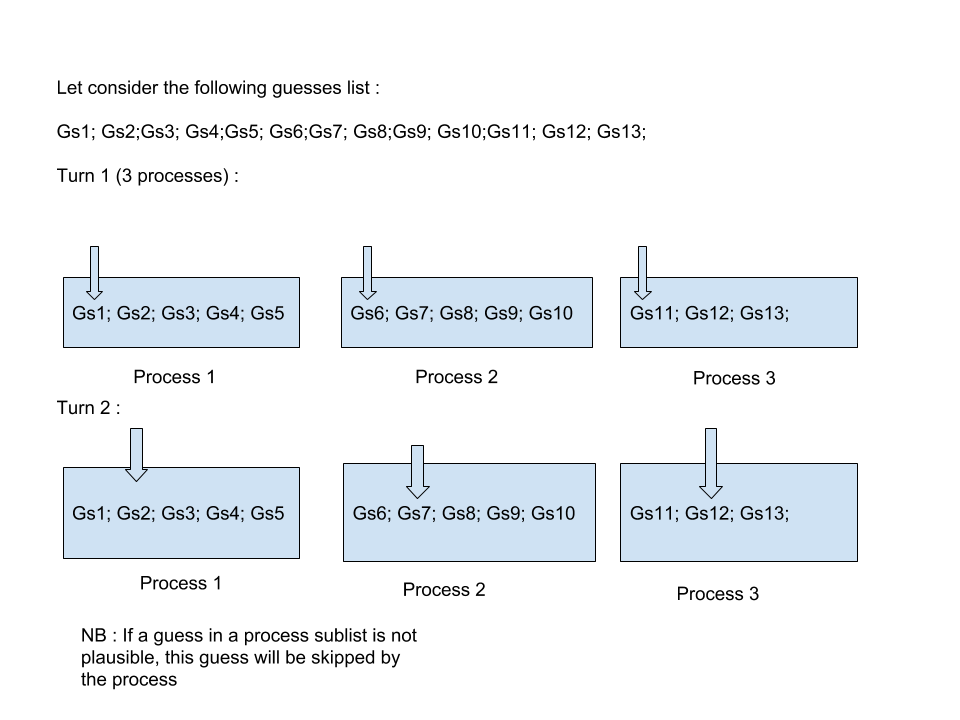
\includegraphics[width=15cm] {pTask.png}
	    \caption{Maximum number of colors }
	    \label{plot12}
	\end{figure}
	
	
\subsection{Criteria for comparing two evaluation}
An evaluation is a pair of two integers: $perfect$ and $colourOnly$. To determine the best 
between two evaluation we take the one with a higher number of $perfect$. If $perfect$s are equals
we take the higher $colourOnly$.

\subsection{Choice of int $size_t$ instead of Int}
To represent colors, we decided to not use interger data type but to use int $size_t$ because int $size_t$ provide more colors choices than Int.\\
The following graph shows the maximum numbers of possible colors using int $size_t$ : 

        \begin{figure}[H]
	    \centering
	    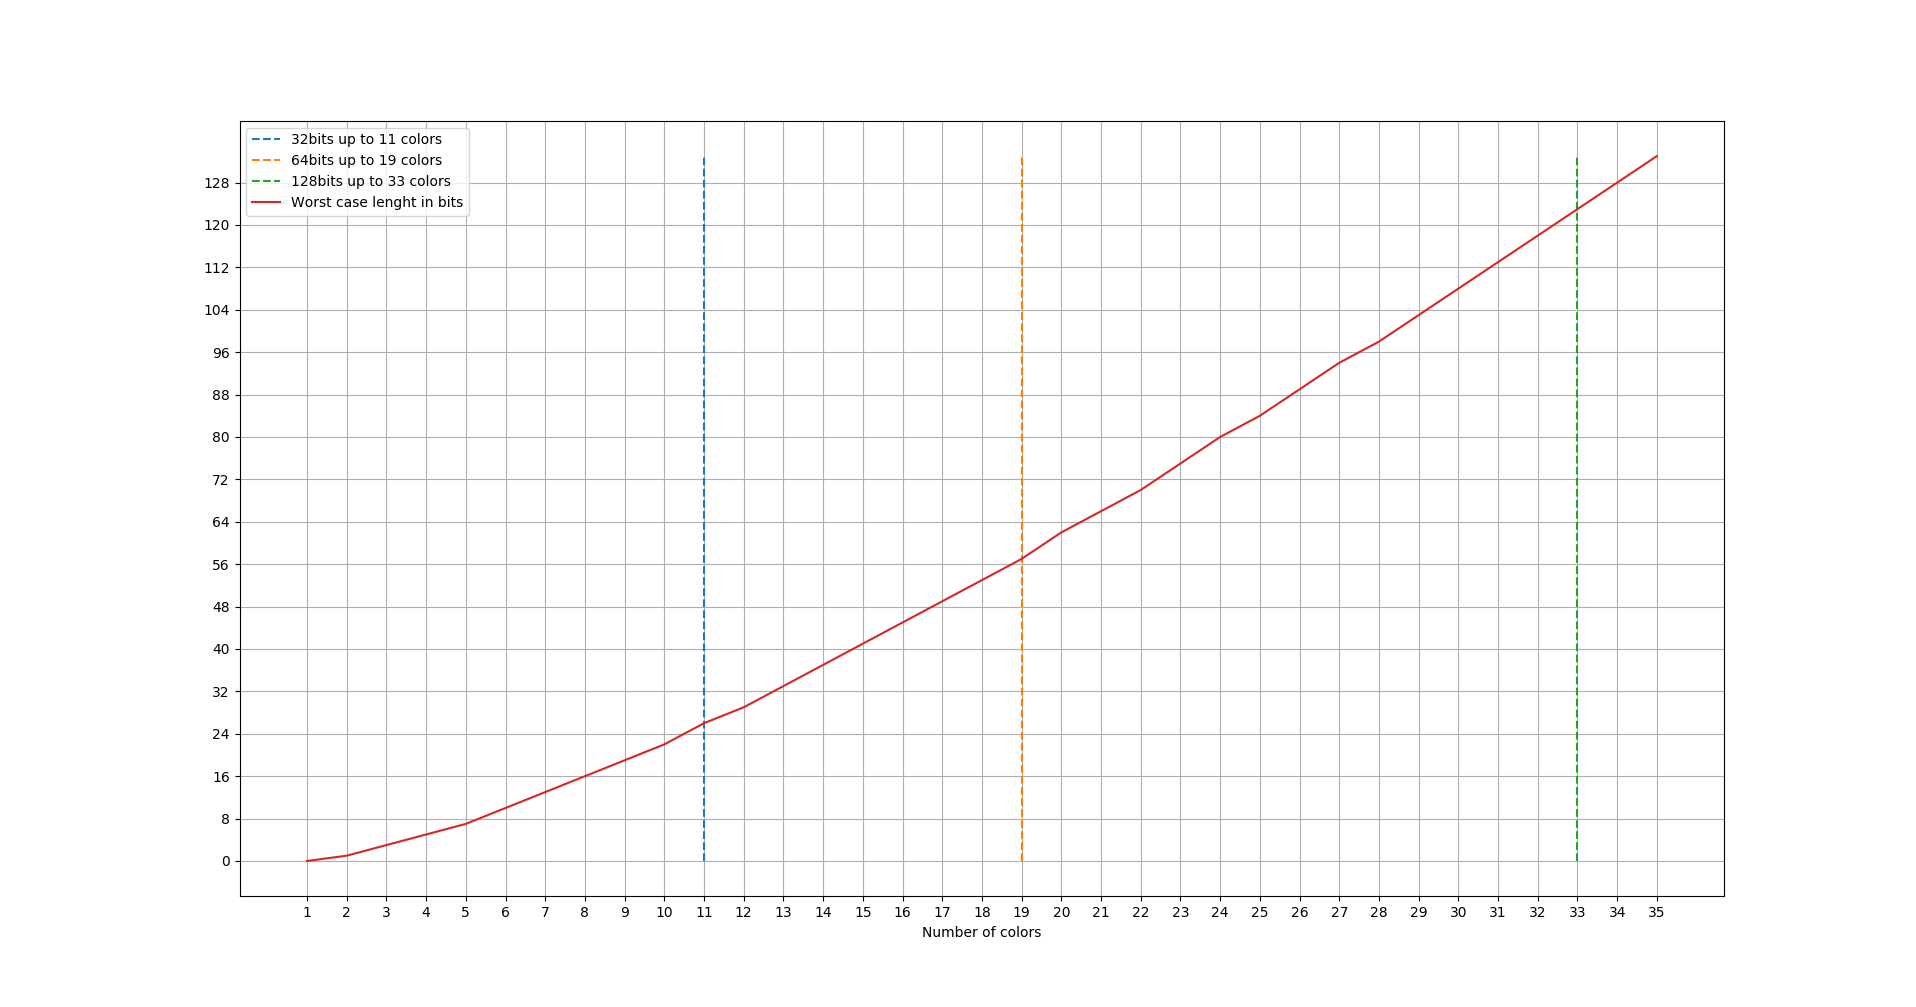
\includegraphics[width=15cm] {maxColors.png}
	    \caption{Maximum number of colors }
	    \label{plot12}
	\end{figure}

\section{MPI Protocal used}
In our project we decide to us two MPI protocols, firstly the MPI Gather and secondly the MPI BCast. \\
We used the MPI Gather in order to get from the game master all the guess that players node generate therefore the master's receive buffer size at each turn  was equal to the spot's number * the number of process. 
        \begin{figure}[H]
	    \centering
	    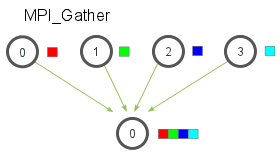
\includegraphics[width=8cm] {gather.png}
	    \caption{MPI Gather }
	    \label{plot12}
	\end{figure}

Secondly we used MPI BCast in order to send a guess and its evaluation to all player's node.

        \begin{figure}[H]
	    \centering
	    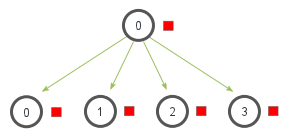
\includegraphics[width=8cm] {bcast2.png}
	    \caption{MPI BCast  }
	    \label{plot12}
	\end{figure}

\section{Class diagram}	

\begin{figure}[H]
	\centering
	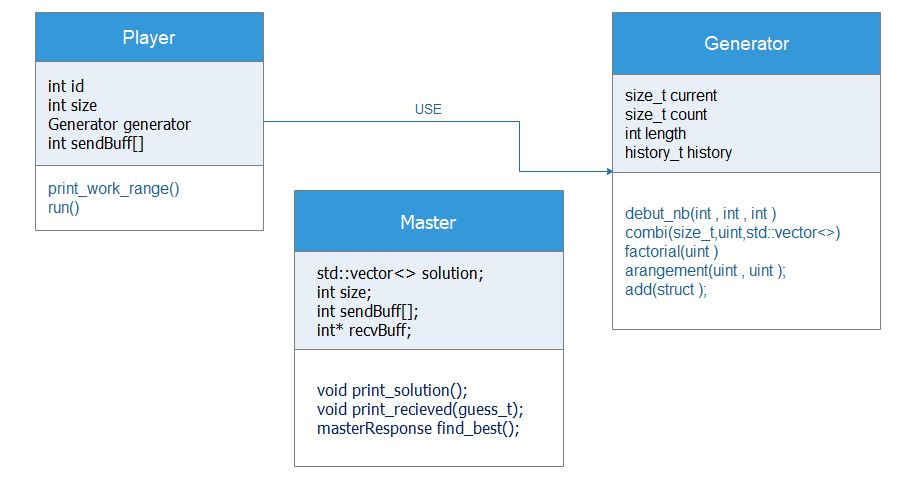
\includegraphics[width=15cm] {classDiag.JPG}
	\caption{Class diagram  }
	\label{plot12}
\end{figure}
\section{Performances and Limitations}
About our code performances and limitations we observed after several running that, the solution was found in at most 6 turn for a sport range of 6 and color range of 15. We also observed that our algorithm end in at most 25 seconds for those range also. \\
One big limitation of our algorithm is the fact that, if the number of spots and colors became huge the speed of our algorithm will decrease proportionally and resources needed will grows also. 


\section{Formula giving the number of possible guesses at start depending on spots and 
colors number}
Let call S the spots number, C the colors number and P the set of plausible guesses at each turn. \\
The following formula give the number of possible guesses at start depending on spots and 
colors number : \\
$ \frac{C!}{(C-S)!}$ - P

\\
\textbf{Note :} The P set can be easily calculate by doing an evaluation between a new guess and previous guesses.

\section{Difficulties during project implementation}
\subsection{Plausible Guess}
During the project a big difficulty that we met was to understand, the concept of plausible guess and how to implement it in our source code.  To overcome this problem we decide to download on our personal cell phones the mastermind game and to try to understand this notion.
\subsection{Hydra message protocol}
As hydra was something new to us, it wasn't something easy for us to understand directly how hydra's message protocols works. This problem were solved by simply reading the file available on UV and by practicing. 


\section{Personal critics on parallel algorithm}
We discover that parallelization was a powerfull method because it allows us to split a task into several nodes and therefore to speed up the time needed for solving the initial problem but we observed also that parallelization has costs such as :
\begin{enumerate}
    \item Sometimes not all processors are used, this can happen because of the intrinsic sequential nature of a given step or part of the problem.
    \item Parallel algorithm are harder to design 
    \item Delays of the communication 
\end{enumerate}

\section{Conclusion}
As said in the introduction, we build multi-processes algorithm for solving the mastermind game. This project helped us to understand deeply how multi-processing and parallelization works. The project allowed us also to see, how powerful can be this method but it also revealed us limitations of parallelization.

\section{Sources}
Google images : 
\begin{enumerate}
    \item  \href{https://www.google.com/search?q=mpi+gather&source=lnms&tbm=isch&sa=X&ved=0ahUKEwiux-DMh5$_$fAhVQbFAKHX87DsUQ$_$AUIDigB&biw=1366&bih=695#imgrc=wk5b6Rw6eXn95M:}{MPI Gather Image}.
    
    \item \href{https://www.google.com/search?q=mpi+gather&source=lnms&tbm=isch&sa=X&ved=0ahUKEwiux
-DMh5_fAhVQbFAKHX87DsUQ_AUIDigB&biw=1366&bih=695#imgrc=WAJ80qLx2p9dvM:}{MPI BCast Image}
\end{enumerate}

\end{document}